\documentclass[smallextended]{svjour3} 
\smartqed
\journalname{New Generation Computing}
\usepackage{cmap}

%\usepackage[utf8]{inputenc}
%\usepackage[T2A]{fontenc}

\usepackage{amssymb,amsfonts}%,amsthm,amsmath}
\usepackage{mathtext,enumerate,float}
%\usepackage[russian, english]{babel}
%\usepackage{graphicx}
\usepackage{tabularx}

%\usepackage{enumerate}
%\usepackage{fancyhdr}
%\usepackage{a4wide}
%\usepackage{cite}

\usepackage{caption}
\usepackage[caption=false]{subfig}
%\usepackage{multicol}

\usepackage{mathtools}
\sloppy
%\renewcommand{\headrulewidth}{0pt}
\DeclareMathOperator*{\argmin}{arg\,min}
\DeclareMathOperator*{\argmax}{arg\,max}
\DeclarePairedDelimiter\ceil{\lceil}{\rceil}
\DeclarePairedDelimiter\floor{\lfloor}{\rfloor}

\begin{document}

%\begin{frontmatter}


%\title{Comprehensive analysis of gradient-based hyperparameter optimization algorithms\footnote}
%\date{}
%\maketitle

% \begin{center}
% {O.\,Y.~Bakhteev\footnote{Moscow Institute of Physics and Technology, bakhteev@phystech.edu},
% V.\,V.~Strijov$^1$\footnote{FRCCSC of the Russian Academy of Sciences, strijov@ccas.ru}} % основной список авторов, выводимый в оглавление
% \end{center}

\title{Comprehensive analysis of gradient-based hyperparameter optimization algorithms\thanks{The research was made possible by Government of the Russian Federation (Agreement № 05.Y09.21.0018)}}% \tnoteref{label1}}
%\tnotetext[label1]{The research was made possible by Government of the Russian Federation (Agreement № 05.Y09.21.0018)}

\author{O.\,Y.~Bakhteev        \and
        V.\,V.~Strijov %etc.
}

\institute{O.\,Y.~Bakhteev \at
              Moscow Institute of Physics and Technology \\
              Tel.: +74991354163\\             
              \email{bakhteev@phystech.edu}           %  \\
%             \emph{Present address:} of F. Author  %  if needed
           \and
           V.\,V.~Strijov \at
              Moscow Institute of Physics and Technology 
            \and 
            FRCCSC of the Russian Academy of Sciences
}

\date{Received: date / Accepted: date}
% The correct dates will be entered by the editor


\maketitle



%\author[mipt]{O.\,Y.~Bakhteev \corref{cor1}}
%\ead{bakhteev@phystech.edu}

%\author[mipt,vc]{V.\,V.~Strijov}
%\ead{strijov@ccas.ru}
%\cortext[cor1]{Corresponding author}
%\address[mipt]{Moscow Institute of Physics and Technology}
%\address[vc]{FRCCSC of the Russian Academy of Sciences}

%% \author{Name\corref{cor1}\fnref{label2}}
%% \ead{email address}
%% \ead[url]{home page}
%% \fntext[label2]{}
%% \cortext[cor1]{}
%% \address{Address\fnref{label3}}
%% \fntext[label3]{}


\begin{abstract} 
%The paper investigates the problem of hyperparameter optimization problem for models with large number of parameters.
%For this problem solution the paper proposes gradient-based algorithms. For the model selection propose probabilistic interpretation of parameter distribution. The paper compares two model selection criterion: cross-validation and evidence lower bound that is a lower bound of marginal likelihood. The experiment is conducted on a series of datasets.\bigskip

%The paper investigates the problem of hyperparameter optimization problem.
%The paper analyzes gradient-based algorithms of hyperparameter optimization: HOAG, DrMad and greedy algorithm.  The complexity of the parameter optimization is comparable to the hyperparameter optimization complexity, therefore  optimize the model parameters and hyperparameters is a single procedure. The paper compares two model selection criterion: cross-validation and evidence lower bound that is a lower bound of marginal likelihood. 
The paper investigates  hyperparameter optimization problem. Hyperparameters are the parameters of model parameter distribution. The adequate choice of hyperparameter values prevents model overfit and allows it to obtain higher predictive performance.  Neural network models with large amount of hyperparameters are analyzed. The hyperparameter optimization for models is computationally expensive. The paper proposes modifications of various gradient-based methods to simultaneously optimize many hyperparameters. The paper compares the experiment results with the random search. The main impact of the paper is hyperparameter optimization algorithms analysis for the models with high amount of parameters. To select precise and stable models the authors suggest to use two model selection criteria: cross-validation and evidence lower bound. The experiments show that the models optimized using the evidence lower bound give higher error rate
than the models obtained using cross-validation. These models also show greater stability when data is noisy.  The evidence lower bound usage
is preferable when the model tends to overfit or when the cross-validation is computationally expensive. The algorithms are evaluated on  regression and classification datasets.


\keywords{gradient descent \and  hyperparameter optimization \and model selection \and neural networks \and classification \and regression}
%\begin{keyword}  gradient descent, stochastic hyperparameter search, hyperparameter optimization, model selection, neural networks, classification, regression.
%\end{keyword}
%\end{frontmatter}
\end{abstract}
\section{Introduction}
\label{intro}
The paper analyzes hyperparameter optimization problem. \textit{Model} is a function superposition, which solves a classification or regression problem. \textit{Model hyperparameters} are the parameters of model parameter distribution.

The paper focuses on the neural network models. The parameter optimization problem is computationally expensive because of training loss non-convexity. The amount of model parameters can reach millions~\cite{hinton_rbm}  and such models optimization requires multiple days\cite{suts}.   The hyperparameter values can influence significantly the quality of models~\cite{journal1,journal2}. These two facts make the hyperparameter optimization problem very important. The adequate choice of hyperparameter values also helps to prune redundant parameters to make the model more compact and stable~\cite{nips,ard}.

In this paper gradient-based algorithms are analyzed. They optimize a large amount of hyperparameters within a short time in contrast to gradient-free algorithms~\cite{hyper}.  The complexity of hyperparameter optimization is comparable to the model parameter optimization complexity, therefore, the parameters and hyperparameters are  optimized in a single procedure. As a baseline, a random search algorithm is used. The pros and cons of all the algorithms  
are illustrated in Table~\ref{table:algo_descr}. Opposing to papers~\cite{hyper_mad,hyper_hoag,hyper_greed} this research does not focus on the hold-out cross-validation and analyzes algorithms in general. The analyzed algorithms are implemented as a toolbox~\cite{pyfos}. The authors propose a number of analyzed algorithms modifications: we extend all the algorithms to work with validation loss that can contain hyperparameters, for DrMad algorithm~\cite{hyper_mad} we add an additional parameter that regularizes a length of analyzed parameter update trajectory, for HOAG algorithm~\cite{hyper_hoag} we use stochastic gradient descent for large linear system solving because of high dimension of the linear system.   The main theoretical impact of the paper is the analysis of algorithm behavior with various validation loss functions and a quality and stability analysis of the resulting models. The experiments were conducted using cross-validation and evidence lower bound as a model selection criterion. Opposing to the paper~\cite{hyper_hoag}, where  the optimization algorithms comparison can also be found, this paper presents the results on the large datasets, such as  WISDM~\cite{wisdm} and MNIST~\cite{mnist}, where the number of hyperparameters is significant. 
The experimental results show that the gradient-based algorithms are significantly more effective when the number of hyperparameters is large. 

\begin{table}
\footnotesize
% Алгоритм & Тип алгоритм & Время & Плюсы & Минусы 

\begin{tabularx}{\textwidth}{|p{2cm}|p{2cm}|X|X|}
\hline
\bf Algorthm & \bf Type  & \bf Pros & \bf Cons  \\ \hline
Random search & Stochastic & Easy to implement & Ineffective in high dimensions (curse of dimension)\\ \hline
Greedy~\cite{hyper_greed} & Gradient-based & Can be used in inner model parameter optimization& Greedy and non-optimal: the algorithm is correct whenever the loss function Hessian is identical. \\ \hline
HOAG~\cite{hyper_hoag} & Gradient-based & Fast convergence & The algorithm requires additional parameter configuration: it is required to solve the linear system, which depends on the Hessian of a loss function. The error in linear system solution influences the final model quality.\\ \hline 
DrMAD~\cite{hyper_mad} & Gradient-based & Considers the trajectory of parameter updates and the optimization algorithm.& Can be instable because of gradient explosion or vanishing. The algorithm is correct when the trajectory of parameter update is linear, which is mostly not true for the complex non-convex models. \\ \hline
\end{tabularx}

\caption{The analyzed algorithms properties.}
\label{table:algo_descr}

\end{table}


\paragraph{Related works.}
The papers~\cite{random1,random2} propose hyperparameters optimization strategies based on the random search. The current gold-standard methods~\cite{probopt1,probopt2}   propose hyperparameter optimizations based on the probabilistic models construction for the optimal hyperparameter value prediction. These methods are  ineffective whenever the number of hyperparameters is large~\cite{hyper}.

In~\cite{hyper,hyper2,hyper_mad,hyper_hoag,hyper_greed} the gradient-based hyperparameter optimization methods are suggested. The papers~\cite{hyper_mad,hyper} propose the gradient-based methods that use reverse differentiation method. This method is similar to backpropagation. The main idea of this approach is to restore the full history of parameter updates in order to optimize hyperparameters using this history. In general this procedure is computationally expensive. In~\cite{hyper_greed} the authors propose to use only the last update of parameters at each optimization iteration. This method can be considered as a greedy hyperparameter optimization algorithm. In~\cite{hyper}  the model parameters are optimized using stochastic gradient descent with momentum, which allows to use less memory for storing the parameter update history. In~\cite{hyper_mad} propose to linearize the history trajectory to effectively restore the update history. In~\cite{hyper_hoag} use an approximation of the exact hyperparameter gradient, which can be calculated when the problem satisfies some regular conditions.

For the hyperparameter optimization various model selection criteria can be used~\cite{MacKay,Bishop}. 
In~\cite{MacKay,Bishop,tokmakova,strijov_dsc}  marginal likelihood or \textit{evidence} is used. In~\cite{tokmakova,strijov_dsc} the authors consider the problem of model selection and hyperparameter optimization for the linear regression problem. One of  the marginal likelihood approximation methods is an \textit{evidence lower bound}, which can be obtained using variational inference~\cite{Bishop}. In~\cite{hoffman} a stochastic version of the variational inference is proposed. In~\cite{varmc} the authors analyze the relation between the gradient-based evidence lower bound estimations and MCMC methods. An alternative model selection criterion is a minimum description length~\cite{mdl} that characterizes statistical complexity of the model. In~\cite{nips} an evidence lower bound estimation method for the neural networks is proposed. The authors analyze the relation between the evidence lower bound and minimum description length. 

The other model selection criterion is the cross-validation~\cite{cv_ms,tokmakova}. One of this criterion problem  is its high computational cost~\cite{expensive,expensive2}. In~\cite{bias,bias2} the authors analyze the variance of cross-validation model performance estimation. In~\cite{tokmakova} the authors compare hyperparameter values obtained during hyperparameter optimization using various model selection criteria.



\section{Problem statement}
\label{prob_stat}
There is given a dataset \begin{equation}\label{eq:dataset}\mathfrak{D} = \{(\mathbf{x}_i,y_i)\}, i = 1,\dots,m.\end{equation} It contains the object matrix $\mathbf{X}$ and the label vector  $\mathbf{y}$. The label  ${y_i}$ is in finite set, ${y}_i \in \mathbb{Y} = \{1, \dots, Z\}$, in case of $Z$-class classification problem. For the regression problem the label $y_i$ is in the real-value subset ${y_i} \in \mathbb{Y} \subset  \mathbb{R}$.

A model $f$ predicts the variable~$y_i$:
\[
	f:\mathbb{R}^n \to \mathbb{Y}, \quad \mathbf{w} \in \mathbb{R}^u.
\]
It is differentiable with respect to parameters.

Introduce the probabilistic interpretation of the model $f$ for the classification and regression problems.

\paragraph{Regression problem.}
Suppose the dependent variable $y$ is normally distributed:
\begin{equation}
\label{eq:reg}
\mathbf{y} = \mathcal{N}\bigl(\mathbf{f}, \mathbf{I}\bigr),\quad \text{where }\mathbf{f} = \mathbf{f}(\mathbf{w}, \mathbf{X}).
\end{equation}


Define the likelihood function $p(\mathbf{y}|\mathbf{X}, \mathbf{w})$:
\[
	\text{log}p(\mathbf{y}|\mathbf{X}, \mathbf{w}) =-\frac{m}{2}\text{log}(2\pi)   -\frac{1}{2}\bigl(\mathbf{y} - \mathbf{f}(\mathbf{w}, \mathbf{X}))^\mathsf{T}\mathbf{I}(\mathbf{y} - \mathbf{f}(\mathbf{w}, \mathbf{X})\bigr).
\] 

\paragraph{Classification problem.}
For the 2-class classification problem suppose the dependent variable $y$  is distributed binomially:
\begin{equation}
\label{eq:cl}
	\mathbf{y} = \mathcal{B}\bigl(1-\mathbf{f}, \mathbf{f}\bigr),
\end{equation}
where  $\mathbf{f}$ is the probability that objects from the matrix $\mathbf{X}$  belong to the first class.
For the multiclass classification problem the  dependent variable $y$  is distributed multinomially and $r$-th component ${f}_r$ is the probability that objects from the matrix $\mathbf{X}$  belong to the class $r$. Define the likelihood function
\[
	\text{log}p(\mathbf{y}|\mathbf{X}, \mathbf{w}) = \sum_{\mathbf{x}, y \in \mathbf{X}, \mathbf{y}} \sum_{r=1}^Z[y=r] \text{log}{f}_r(\mathbf{w}, \mathbf{x}).
\] 

For both classification~\eqref{eq:cl} and regression~\eqref{eq:reg} problems define the prior distribution~$p(\mathbf{w}|\mathbf{A})$:
\begin{equation}
\label{eq:prior}
	\mathbf{w} \sim \mathcal{N}(\mathbf{0}, \mathbf{A}^{-1}),
\end{equation}
where  $\mathbf{A}^{-1} = \text{diag}[\alpha_1, \dots, \alpha_u]^{-1}$ is the covariance  diagonal matrix. The hypotheses~\eqref{eq:reg},~\eqref{eq:cl} and~\eqref{eq:prior} 	do	not	contradict	each other since the normal distribution is unbounded~\cite{bayes_constr}.  

%Model selection methods consider not only the model parameters $\mathbf{w}$, but also information about the posterior distribution $p(\mathbf{w}|\mathbf{X}, \mathbf{y}, \mathbf{A})$. Therefore distinct the model parameters vector $\mathbf{w}$ and vector of parameters for model selection $\boldsymbol{\theta}$. These vectors can be equal in simple case, when the true positerior distribution $p(\mathbf{w}|\mathbf{X}, \mathbf{y}, \mathbf{A})$ estimation is available or when the model predictive performance is evaluated using only one instance of model parameters. 

Since the high dimensionality  of parameter space and loss functions non-convexity some model selection methods use parameters of multiple models instances. The authors denote  a vector of model parameters by $\mathbf{w}$ and by $\boldsymbol{\theta} \in \mathbb{R}^s$ a vector of parameters for multiple instances or model parameters distribution. The details of $\boldsymbol{\theta}$ construction are given in the model selection methods description.

Introduce an example of hyperparameter optimization using the coherent Bayesian inference. Optimize model parameters $\boldsymbol{\theta} = \mathbf{w}$ according to the model parameter distribution $p(\mathbf{w}|\mathbf{X}, \mathbf{y}, \mathbf{A})$:
\begin{equation}
\label{eq:bayes1}
\hat{\boldsymbol{\theta}} = \argmax \bigl(-L(\boldsymbol{\theta}, \mathbf{A})\bigr) = p(\mathbf{w}|\mathbf{X}, \mathbf{y}, \mathbf{A}) = \frac{p(\mathbf{y}|\mathbf{X},\mathbf{w})p(\mathbf{w}|\mathbf{A})}{p(\mathbf{y}|\mathbf{X},\mathbf{A})}.
\end{equation}

Calculate the hyperparameter  $\mathbf{A}$ posterior distribution:
\[
p(\mathbf{A}|\mathbf{X}, \mathbf{y}) \propto p(\mathbf{y}|\mathbf{X},\mathbf{A})p(\mathbf{A}),
\]
where $\propto$ means proportionality.

Suppose $p(\mathbf{A})$ is uniform on a large interval. The hyperparameter optimization problem is:
\begin{equation}
\label{eq:bayes2}
	Q(\boldsymbol{\theta}, \mathbf{A}) = p(\mathbf{y}|\mathbf{X},\mathbf{A}) = \int_{\mathbf{w} \in \mathbb{R}^u} p(\mathbf{y}|\mathbf{X}, \mathbf{w}) p(\mathbf{w}|\mathbf{A}) \to \max_{\text{diag}(\mathbf{A}) = [\alpha_1, \dots, \alpha_u] \in \mathbb{R}^{n}}.
\end{equation}


%\begin{figure}
%  \includegraphics[width=0.8\linewidth]{slide_plots/hyper.png}
%\label{fig:hyper}
%    \caption{Marginal likelihood dependency on hyperparameter $\alpha$ disrtribution. TODO: переделать}
 
   
%    \end{figure}


Formulate the hyperparameter optimization problem. Given functions $L$ and $Q$ that characterize the model selection method. The loss function $L$ optimizes parameters $\boldsymbol{\theta}$. The validation function $Q$ evaluates the model predictive performance.
The problem is to optimize the parameters $\boldsymbol{\theta}$ and the hyperparameters $\mathbf{A}$: 
\begin{equation}
\label{eq:main}
	\hat{\mathbf{A}} = \argmax_{[\alpha_1, \dots, \alpha_u] \in \mathbb{R}^n} Q(\hat{\boldsymbol{\theta}}(\mathbf{A}), \mathbf{A}),
\end{equation}
\begin{equation}
\label{eq:main2}
	\hat{\boldsymbol{\theta}}(\mathbf{A}) =  \argmin_{\boldsymbol{\theta} \in \mathbb{R}^s} L(\boldsymbol{\theta}, \mathbf{A}).
\end{equation}

Introduce the functions $L, Q$ and $\boldsymbol{\theta}$ for various model selection methods.

\paragraph{Basic method.}
Optimize the model parameters $\boldsymbol{\theta}$ and hyperparameters $\mathbf{A}$ using the whole dataset $\mathfrak{D}$ and the same function for both optimization and model evaluation with one model instance, $L = -Q$:
\begin{equation} 
\label{eq:basic}
Q(\boldsymbol{\theta}, \mathbf{A}) = -L(\boldsymbol{\theta}, \mathbf{A})  = \text{log}p(\mathbf{y}, \mathbf{w} | \mathbf{X}, \mathbf{A}) = \text{log} p(\mathbf{y}|\mathbf{X}, \mathbf{w})+\text{log}p(\mathbf{w}|\mathbf{A}).
\end{equation}

Describe two model selection methods that prevent model overfitting.

\paragraph{Cross-validation.}
Split the dataset  $\mathfrak{D}$ into $k$ equal parts:
$
\mathfrak{D} = \mathfrak{D}_1 \sqcup \dots \sqcup \mathfrak{D}_k.
$


Run $k$ model optimizations for each subset. The vector $\boldsymbol{\theta}$ is a concatenation of model parameters $\mathbf{w}_k$ for each optimization instance:
\[
\boldsymbol{\theta} = [\mathbf{w}_1, \dots, \mathbf{w}_k].
\]
 
Construct the loss function $L$ as an average negative log posterior probability over the remaining part of each split $\mathfrak{D}_1, \dots, \mathfrak{D}_k$:  
\begin{equation}
\label{eq:cv}
L(\boldsymbol{\theta}, \mathbf{A}) = -\frac{1}{k}\sum_{c=1}^k \bigl(\frac{k}{k-1}\text{log}p(\mathbf{y} \setminus \mathbf{y}_c|\mathbf{X}\setminus \mathbf{X}_c, \mathbf{w}_c) + \text{log}p(\mathbf{w}_c|\mathbf{A})\bigr).
\end{equation}

Construct the validation function $Q$ as an average log likelihood over $k$ splits:
\[
Q(\boldsymbol{\theta}, \mathbf{A}) = \frac{1}{k}\sum_{c=1}^k k\text{log}p(\mathbf{y}_c|\mathbf{X}_c, \mathbf{w}_c).
\]

\paragraph{Evidence Lower Bound.}
As in the basic method description let $L=-Q$. It is an evidence lower bound:
\begin{equation} 
\label{eq:elbo}
\text{log}~p(\mathbf{y}|\mathbf{X},\mathbf{A})  
\geq 
-\text{D}_\text{KL} \bigl(q(\mathbf{w})||p(\mathbf{w}|\mathbf{A})\bigr) + \int_{\mathbf{w}} q(\mathbf{w})\text{log}~{p(\mathbf{y}|\mathbf{X},\mathbf{w},\mathbf{A})} d \mathbf{w}  \approx
\end{equation}
\[
\approx \sum_{i=1}^m \text{log}~p({y}_i|\mathbf{x}_i, \mathbf{w}_i) - D_\text{KL}\bigl(q (\mathbf{w}) || p (\mathbf{w}|\mathbf{A})\bigr) = -L(\boldsymbol{\theta}, \mathbf{A}) = Q(\boldsymbol{\theta}, \mathbf{A}),
\]
where $q$ is an auxiliary distribution called variational distribution. Let $q$ be a normal distribution:
\begin{equation}
\label{eq:diag}
	q \sim \mathcal{N}(\boldsymbol{\mu}_q, \mathbf{A}^{-1}_q),
\end{equation}
where $\mathbf{A}_q = \text{diag}[\alpha^q_1, \dots, \alpha^q_u]^{-1}$ is  a diagonal covariance matrix and $\boldsymbol{\mu}_q$ is a mean vector.
The divergence $D_\text{KL}$ between 2 Gaussian variables is 
\[
	D_\text{KL}\bigl(q (\mathbf{w}) || p (\mathbf{w}|\mathbf{f})\bigr) = \frac{1}{2} \bigl( \text{Tr} [\mathbf{A}\mathbf{A}^{-1}_q] + (\boldsymbol{\mu} - \boldsymbol{\mu}_q)^\mathsf{T}\mathbf{A}(\boldsymbol{\mu} - \boldsymbol{\mu}_q) - u +\text{ln}~|\mathbf{A}^{-1}| - \text{ln}~|\mathbf{A}_q^{-1}| \bigr).
\]
The vector of optimized parameters $\boldsymbol{\theta}$ is a vector of variational distribution $q$ parameters:
\[
\boldsymbol{\theta} = [\text{diag}(\mathbf{A}_q), {\mu}_1,\dots,{\mu}_u].
\]




\section{Gradient-based hyperparameter optimization methods}
\label{gbhom}
In this section we analyze hyperparameter optimization methods based on gradient descent. Suppose the parameters $\boldsymbol{\theta}$ are also optimized using gradient-based methods. 

%\newdefinition{dfn}{Definition}
\begin{definition}
A stochastic gradient descent operator $T$ estimates the parameters $\boldsymbol{\theta}^\prime$ using their previous values~$\boldsymbol{\theta}$ with random subset of dataset:
\[
	\boldsymbol{\theta}^\prime = T(\boldsymbol{\theta}, \mathbf{A}, \mathfrak{D}) = \boldsymbol{\theta} - \gamma \nabla L(\boldsymbol{\theta}, \mathbf{A})_{\mathfrak{D} = \hat{\mathfrak{D}}},
\]
where $\hat{\mathfrak{D}}$ is a random subset of $\mathfrak{D}$.
\end{definition}

Optimize the parameters  $\boldsymbol{\theta}$ with $\eta$ steps of stochastic gradient descent:
\begin{equation}
\label{eq:gd}
	 \hat{\boldsymbol{\theta}} = T \circ T \circ \dots \circ T(\boldsymbol{\theta}_0, \mathbf{A}) = T^\eta(\boldsymbol{\theta}_0, \mathbf{A}), \quad 	T(\boldsymbol{\theta}, \mathbf{A}) =\boldsymbol{\theta} - \gamma \nabla L(\boldsymbol{\theta}, \mathbf{A}), 
\end{equation}
where $\gamma$ is the learning rate, $\boldsymbol{\theta}_0$ is the initial values of the vector $\boldsymbol{\theta}$. 

Redefine the optimization problem according to the definition of operator $T$:
\begin{equation}
\label{eq:optim}
	\hat{\mathbf{A}} = \argmax_{\text{diag}(\mathbf{A}) \in \mathbb{R}^n} Q\bigl( T^\eta(\boldsymbol{\theta}_0, \mathbf{A})\bigr).
\end{equation}
Solve the optimization problem~\eqref{eq:optim} using gradient-based methods. The exact gradient calculation $\nabla_{\mathbf{A}} Q( T^\eta(\boldsymbol{\theta}_0, \mathbf{A}))$ is intractable because of the inner optimization operator $T$. The scheme of the hyperparameter optimization.
\begin{enumerate}
\item In range from 1 to  $l$, where $l$ is the number of the hyperparameter optimization iterations:
\item Initialize parameters $\boldsymbol{\theta}$.
\item Solve optimization problem~\eqref{eq:optim} and obtain the new hyperparameter values $\mathbf{A}'$
\item Set $\mathbf{A} = \mathbf{A}'$.
\end{enumerate}

Introduce methods of numerical solution for this optimization problem. Their main properties are listed in Table~\ref{table:algo_descr2}.

\begin{table}
\small

% Алгоритм & Тип алгоритм & Время & Плюсы & Минусы 

\begin{tabularx}{\textwidth}{|X|X|X|X|}
\hline
\bf Algorithm & \bf Type & \bf Optimization iteration complexity & \bf Correctness suppositions  \\ 
\hline
Random search & stochastic & $O(\eta u |\hat{\mathfrak{D}}|)$& -  \\ \hline
Greedy~\cite{hyper_greed} & gradient-based & $O(\eta u |\hat{\mathfrak{D}}|)$ & $\mathbf{H}(\boldsymbol{\theta}) = \mathbf{I}$  \\ \hline
HOAG~\cite{hyper_hoag} & gradient-based & $O(\eta u |\hat{\mathfrak{D}}| + \text{o}),$ where $o$ is a complexity of linear equation solution& first derivatives of $Q$  and second derivatives of $L$ are Lipshitz functions;  $\text{det}\mathbf{H} \neq \mathbf{0}$;  \\ \hline
DrMAD~\cite{hyper_mad} & gradient-based &$O(\eta u |\hat{\mathfrak{D}}|)$ & Parameter trajectory$\boldsymbol{\theta}$ = $\boldsymbol{\theta}_0, \dots \boldsymbol{\theta}_\eta$  is linear \\ \hline
\end{tabularx}

\caption{The analyzed algorithms complexity and correctness. The model is a multilayer perceptron optimized using backpropagation with the basic model selection method~\eqref{eq:basic}.}
\label{table:algo_descr2}

\end{table}
%Greedy: backprop + optimization. 


\paragraph{Greedy algorithm.}
Update the hyperparameter $\mathbf{A}$ using gradient descent, which depends only on the last update of parameters $\boldsymbol{\theta}$. Optimize the hyperparameters and parameters in a single optimization procedure. Update the hyperparameter $\mathbf{A}$ at every iteration:
\[
	\mathbf{A}' = \mathbf{A} + \gamma_{\mathbf{A}} \nabla_{\mathbf{A}}  Q \bigl(T(\boldsymbol{\theta}, \mathbf{A}) , \mathbf{A}\bigr) = \mathbf{A} + \gamma_{\mathbf{A}} \nabla_{\mathbf{A}}  Q\bigl(\boldsymbol{\theta} - \gamma \nabla L(\boldsymbol{\theta}, \mathbf{A}), \mathbf{A})\bigr),
\]
where $\gamma_{\mathbf{A}}$ is the learning rate for the hyperparameter optimization.

\paragraph{HOAG.}
Obtain approximate hyperparameter gradient values  $\nabla_{\mathbf{A}} Q \bigl(T^\eta(\boldsymbol{\theta}_0, \mathbf{A})\bigr)$ using the following  formula approximation of the  of the gradient:
\[
\nabla_{\mathbf{A}} Q \bigl(T^\eta(\boldsymbol{\theta}_0, \mathbf{A})\bigr) = \nabla_{\mathbf{A}} Q(\boldsymbol{\theta}, \mathbf{A}) - (\nabla_{ \mathbf{A}}  \nabla_{\boldsymbol{\theta}} L(\boldsymbol{\theta}, \mathbf{A}))^\mathsf{T}\mathbf{H}(\boldsymbol{\theta})^{-1}\nabla_{\boldsymbol{\theta}} Q(\boldsymbol{\theta}, \mathbf{A}),
\]
where $\mathbf{H}$ is the Hessian of the function $L$ with respect to the parameters $\boldsymbol{\theta}$.

The algorithm of hyperparameter gradient $\nabla_{\mathbf{A}} Q$  approximation:
\begin{enumerate}
\item Optimize the parameters $\boldsymbol{\theta} = T^\eta(\boldsymbol{\theta}_0, \mathbf{A})$.
\item Solve linear system for a vector $\boldsymbol{\lambda}$: $\mathbf{H}(\boldsymbol{\theta})\boldsymbol{\lambda} =  \nabla_{\boldsymbol{\theta}} Q(\boldsymbol{\theta}, \mathbf{A})$.
\item Compute the approximate hyperparameter gradient: $\hat{\nabla}_{\mathbf{A}}Q = \nabla_{\mathbf{A}}Q(\boldsymbol{\theta}, \mathbf{A}) - \nabla_{ \mathbf{A}}  \nabla_{\boldsymbol{\theta}} L(\boldsymbol{\theta}, \mathbf{A})^\mathsf{T}\boldsymbol{\lambda}$.
\end{enumerate}

The final update rule is
\begin{equation}
\label{eq:update_hyper}
\mathbf{A}' = \mathbf{A} + \gamma_{\mathbf{A}} \hat{\nabla}_{\mathbf{A}}Q.
\end{equation}
The computational cost of the Hessian $\mathbf{H}(\boldsymbol{\theta})$ evaluation  from step 2 is high.  In this paper we use stochastic gradient descent for solving this linear system. 


\paragraph{DrMad.}
For the hyperparameter gradient evaluation restore the full history of $\eta$ parameters updates starting from the initial value $\boldsymbol{\theta}_0$.  For the simplification of this procedure suppose that the trajectory of parameters $\boldsymbol{\theta}$ update is linear:
\begin{equation}
\label{eq:mad_lin}
\boldsymbol{\theta}^\tau = \boldsymbol{\theta}_0 + \frac{\tau}{\eta} T(\boldsymbol{\theta}).
\end{equation}

The algorithm of approximate hyperparameter gradient calculation:
\begin{enumerate}
\item Optimize  parameters $\boldsymbol{\theta} = T^\eta(\boldsymbol{\theta}_0, \mathbf{A})$.
\item Let $\hat{\nabla} \mathbf{A} = \nabla_\mathbf{A} Q(\boldsymbol{\theta}, \mathbf{A}).$ 
\item Let $\hat{\nabla} \boldsymbol{\theta} = \nabla_{\boldsymbol{\theta}} Q(\boldsymbol{\theta}, \mathbf{A}).$ 
%\item Let $d\mathbf{v} = \mathbf{0}.$
\item In range from $\tau = \eta$ to  1:
\item Compute $\boldsymbol{\theta}^\tau$\eqref{eq:mad_lin}.
\item $d\mathbf{v} =  \gamma \hat{\nabla} {\boldsymbol{\theta}}$.
\item $\hat{\nabla} \mathbf{A} =  \hat{\nabla} \mathbf{A} + d\mathbf{v}\nabla_{\mathbf{A}} \nabla_{\boldsymbol{\theta}} L$.
\item $\hat{\nabla} \boldsymbol{\theta}  = \hat{\nabla} \boldsymbol{\theta}  - d\mathbf{v}\nabla_{\boldsymbol{\theta}} \nabla_{\boldsymbol{\theta}} L$.
\end{enumerate}
The final update rule is analogous to~\eqref{eq:update_hyper}.
The algorithm is instable when the learning rate $\gamma$ is large~\cite{hyper_mad}. For the stability of the algorithm we discard first 5\% of values  $\boldsymbol{\theta}$ and calculate only each $\tau_\text{step}$ step of parameter updates history:
\begin{equation}
\label{eq:mad_lin2}
\boldsymbol{\theta}^\tau = \boldsymbol{\theta}_{\tau_0} + \frac{\tau}{\eta} T(\boldsymbol{\theta}), \quad \tau \in \{\tau_0, \tau_o + \tau_\text{step}, \dots,\eta - \tau_\text{step}, \eta\},
\end{equation}
where $\tau_0 = \ceil{0.05 \cdot \eta}$.

\section{Experiments}
\label{experiments}
For the evaluation of the analyzed algorithms we conducted a series of computational experiments. A synthetic dataset, WISDM~\cite{wisdm} and MNIST~\cite{mnist} datasets were used. All datasets were splitted into Train and Test subsets. The  algorithms were evaluated on the Test subsets. For each dataset and each algorithm we ran 5 optimizations. The results were averaged. 
We used the following evaluation criteria.
\begin{enumerate}
\item Quality: the best value of $Q$:  $\hat{Q} = \max_{j \in \{1, \dots, l\}}Q^j$.
\item Convergence: the number of iterations to have a validation value greater than 99\% of the best value $\hat{Q}$:
\[
    \argmin_{j}: \frac{Q^j - Q^0}{\hat{Q} - Q^0} \geq 0.99,
\]
where $Q^0$ is the value of $Q$ before the hyperparameter optimization. 


\item Error function $E$:\[
    E = \text{RMSE}(\mathbf{X}_\text{test}, \mathbf{y}_\text{test}) = \left (\frac{1}{|\mathbf{X}_\text{test}|}\sum_{\mathbf{x} \in\mathbf{X}_\text{test}, y \in \mathbf{y}_\text{test}}  (f(\mathbf{x}, \mathbf{w})-y)\right)^{\frac{1}{2}}
\]
for the regression problem and
\[
    E = \text{Acc}(\mathbf{X}_\text{test}, \mathbf{y}_\text{test}) = 1 - \frac{1}{|\mathbf{X}_\text{test}|}\sum_{\mathbf{x} \in\mathbf{X}_\text{test}, y \in \mathbf{y}_\text{test}} [f(\mathbf{x}, \mathbf{w}) \neq y]
\]
for the classification problem.


\item The error function  $E_\sigma$ for the model with noisy dataset:
\[
    \text{RMSE}_\sigma =  \text{RMSE}(\mathbf{X}_\text{test} +  \boldsymbol{\varepsilon}, \mathbf{y}_\text{test}),\]\[\text{Acc}_\sigma =  \text{Acc}(\mathbf{X}_\text{test} +  \boldsymbol{\varepsilon}, \mathbf{y}_\text{test}),  \quad \boldsymbol{\varepsilon} \sim \mathcal{N}\bigl(\mathbf{0}, \sigma\mathbf{I}\bigr).
\]
\end{enumerate}



The random search was used as a baseline. The number of the random search iterations equaled to the number $l$ of gradient-based hyperparameter optimization algorithms iterations. It was set to $l=50$ for the synthetic dataset and WISDM dataset, $l=25$ for the MNIST dataset.  For the loss  function $L$ and validation function $Q$ cross-validation~\eqref{eq:cv} with $k=4$ and evidence lower bound~\eqref{eq:elbo} were used. 

For the neural network models we set all the hyperparameters equal for each layer when used  cross-validation~\eqref{eq:cv}. The full diagonal parameterization of the hyperparameters was used for all the linear models and for the neurla network models when we used evidence lower bound~\eqref{eq:elbo}.


\begin{figure*}[tbh!]
    \centering
    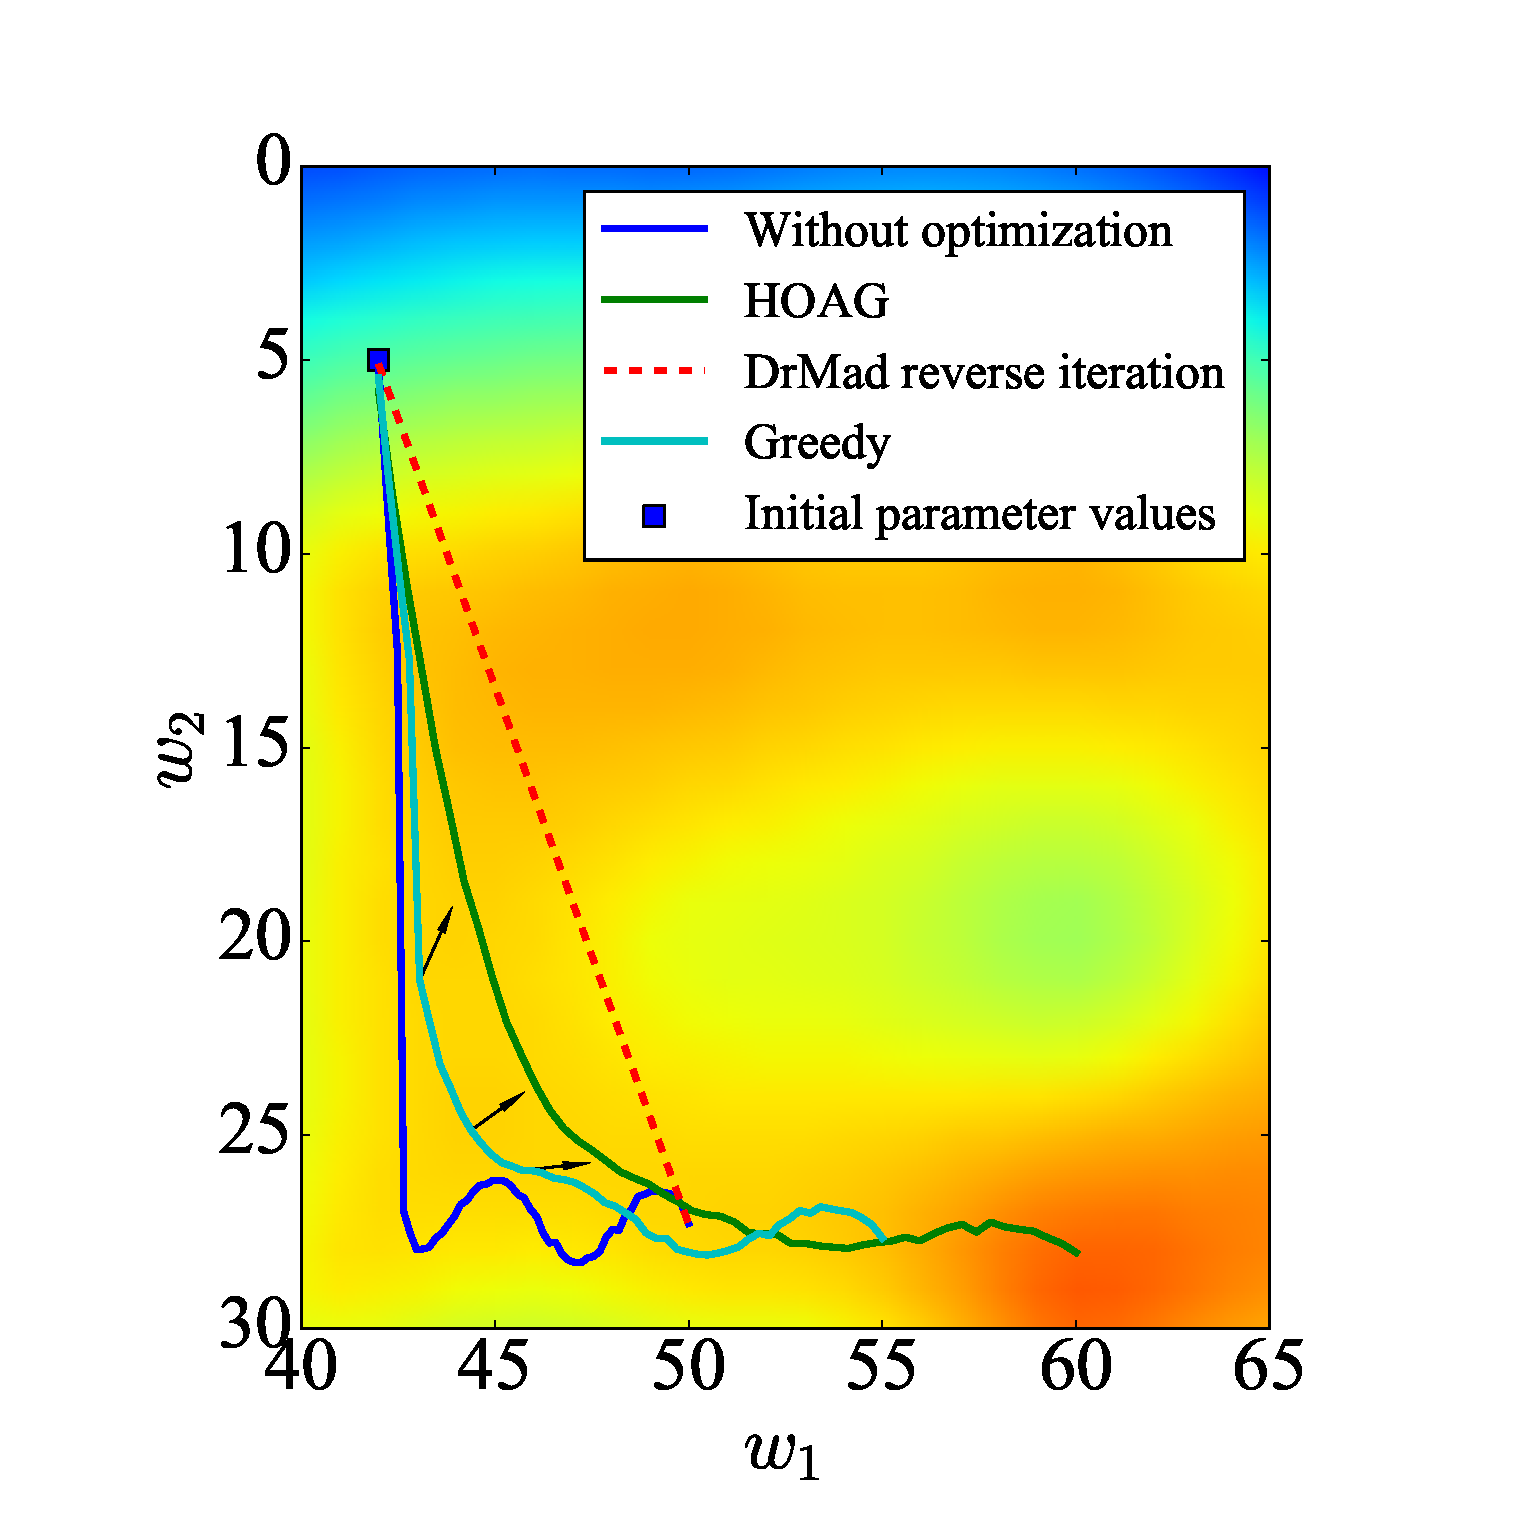
\includegraphics[width=0.5\linewidth]{Fig_traj.eps}

    \caption{An example of parameter update trajectories. The color displays the value of the validation function $Q$. Greedy algorithm optimizes hyperparameter during the parameter optimization, therefore it has the light blue trajectory between the optimized green trajectory of HOAG algorithm and the dark blue trajectory of parameters without hyperparameter optimization. DrMAD uses a linearized dashed parameter trajectory during hyperparameter optimization procedure.  }
    \end{figure*}


The hyperparameters were initialized with uniform distribution $\mathcal{U}(a,b)$,
where $a = -2, b = 10$ for the synthetic dataset and $a = -4, b = 10$  for the WISDM and MNIST datasets.

We calibrated the hyperparameter learning rate $\gamma_{\mathbf{A}}$  for each algoritm using grid search:~$\{r \cdot 10^{s}, s \leq 1, r \in \{1,25,50,75\}\}$. The largest value of $\gamma_{\mathbf{A}}$ was chosen if the final hyperparameter value $\mathbf{A}$ satisfied the condition:
\[
    a_\text{min} \leq  \min(\mathbf{A}), \quad \max(\mathbf{A}) \leq b_\text{max},
\] 
where $a_\text{min} = -2.5, b_\text{max}=10.5$ for the synthetic dataset and $a_\text{min} = -5, b_\text{max}=11$ for the WISDM and MNIST datasets. We calibrated $\gamma_\mathbf{A}$ with a small amount of iterations: $l=50$ for the syntetic dataset, $l=10$ for the WISDM and $l=5$ for the MNIST dataset. Whenever each algorithm showed instability in further experiments (gradient explosion or overflow) the value of $\gamma_{\mathbf{A}}$ was lowered. The parameter $\tau_\text{step}$ set to $1$ for syntetic dataset and WISDM and  $\tau_\text{step}=10$ for the MNIST dataset.



\paragraph{Synthetic dataset.}
The synthetic dataset was generated according to the rule:
\[
	\mathbf{y} = \mathbf{x} + \boldsymbol{\varepsilon},\quad \mathbf{x}  \sim \mathcal{N}(\mathbf{0}, \mathbf{I}) \quad \boldsymbol{\varepsilon} \sim \mathcal{N}(\mathbf{0}, \mathbf{I}),
\]
where $\quad m = 40, \quad n = 1.$

The regression model $\mathbf{f}$ uses the following features: $\{\mathbf{x}^0, \dots, \mathbf{x}^9, \textbf{sin}(\mathbf{x}), \textbf{cos}(\mathbf{x})\}$. The unregularized regression model with this such ratio of  object number and feature number tends to overfit significantly. The goal of this experiment was to analyze if the hyperparameter optimization could protect such models from overfit.

Fig.~\ref{fig:poly} plots the resulting polynoms. 
The evidence lower bound criterion~\eqref{eq:elbo} gave non-overfitted polynoms, which parameters are close to the linear models.

\paragraph{WISDM.}
The WISDM dataset contains a set of records from accelerometer. Each record has three coordinates that correspond to the accelerometer axes. As a set of features we used first 199  records from each 200 sequential records. We used $l_2$ norm of the 200th records as a label and required to predict. 

A neural network with 10 neurons on the hidden layer was used:
\[
    \mathbf{f} = \mathbf{W}_2 \cdot \textbf{RELU}(\mathbf{W}_1\mathbf{x} + \mathbf{b}_1) +\mathbf{b}_2,
\]
where $\mathbf{W}_1, \mathbf{b}_1$ --- hidden layer parameters,
$\mathbf{W}_2, \mathbf{b}_2$ --- output layer parameters,
\[
    \textbf{RELU}(\mathbf{x}) = \max(\mathbf{0}, \mathbf{x}).
\]

Fig.~\ref{fig:wisdm} shows the plots with RMSE and best validation loss value $\hat{Q}$ for the WISDM dataset.
DrMad and HOAG algorithms showed significantly lower results than greedy algorithm. The random search showed good results in case of cross-validation, when the number of hyperparameters is small. When the number of hyperparameters is large the greedy and HOAG algorithm showed good results. HOAG requires more iteration number $l$ than the greedy algorithm for the convergence.


\paragraph{MNIST.}
The MNIST dataset contains a set of images of handwritten digits. 
We used a neural network with 300 neurons on the hidden layer and softmax output.


Fig.~\ref{fig:mnist} plots the error $E$ and quality $\hat{Q}$.
For the evidence lower bound criterion, the models with highest $\hat{Q}$ value have also highest error $E$. Nevertheless, 
these models showed the best results for the stability, when the noise in dataset is high. Fig.~\ref{fig:noise} plots  the error $E_\sigma$. Models with highest evidence lower bound have the lowest error when the Test dataset is noisy. We interpret this as an ability to select the model with highest generalization ability.

As we can see from the experiments, the gradient-based methods give better results than the random search when the number of hyperparameters is large. The best results for all the experiments were obtained by greedy algorithm. DrMad algorithm showed weaker results than greedy and HOAG algorithms because of its instability: the algorithm often had gradient explosions, therefore the learning rate $\gamma_{\mathbf{A}}$ for it was set to low values during calibration. 



\begin{table}
\footnotesize
\begin{tabularx}{\textwidth}{ |X|p{0.75cm}|X|X|p{1cm}|X|X|X|X|}

\hline
\textbf{Algorithm} & $L, Q$  & $Q(\boldsymbol{\theta}, \mathbf{A})$ & Convergence & E & $E_{0.25}$ & $E_{0.5}$\\ 
\hline
\multicolumn{7}{|c|}{\textit{Synthetic}}  \\
\hline
Random search & ~\eqref{eq:cv} & \bf -171.6  &\bf 26.2 $\pm$ 20.0  & \bf 1.367 &\bf 1.410 &\bf 1.555 \\
\hline
Greedy & ~\eqref{eq:cv} & -172.5 & 30.0 $\pm$ 24.5 & 1.421 & 1.439 &  1.536\\
\hline
DrMAD & ~\eqref{eq:cv} & -174.1 & 40.2 $\pm$ 16.1 &  1.403 & 1.424 & \bf 1.512 \\
\hline
HOAG & ~\eqref{eq:cv} &-174.7 & 29.4 $\pm$ 24.0 &   \bf 1.432  & 1.463 & 1.553\\
\hline
Random Search & ~\eqref{eq:elbo} & -63.5  & 32.4 $\pm$ 18.7  & 1.368 & 1.426 & 1.546  \\
\hline
Greedy & ~\eqref{eq:elbo} & -25.5 & \bf 1.2 $\pm$ 0.4 & 1.161 & 1.174 & 1.193\\
\hline
DrMAD & ~\eqref{eq:elbo} & \bf -25.1 &  10.6 $\pm$ 0.8 &  1.157 & 1.163 &  1.184\\
\hline
HOAG & ~\eqref{eq:elbo} &-25.8 & 10.8 $\pm$ 1.5&   \bf 1.141  & \bf 1.149 & \bf 1.177\\
\hline


\multicolumn{7}{|c|}{\textit{WISDM}}  \\
\hline
Random search & ~\eqref{eq:cv} & \bf -1086661.1  & 22.0 $\pm$ 19.3  & \bf 0.660 & \bf 0.670 & \bf 0.690  \\
\hline
Greedy & ~\eqref{eq:cv} & -1086707.1 & \bf 15.4 $\pm$ 17.2 & 0.707 &  0.723  &  0.769\\
\hline
DrMAD & ~\eqref{eq:cv} & -1086708.2 & 29.2 $\pm$ 8.0 &  0.694 &  0.708 & 0.742 \\
\hline
HOAG & ~\eqref{eq:cv} & -1086733.5 & 28.2 $\pm$ 7.13&   0.701 & 0.724 & 0.753 \\
\hline
Random search & ~\eqref{eq:elbo} & -35420.4 &   14.4 $\pm$ 7.8  &   0.732 &   0.755 & 0.785 \\
\hline
Greedy & ~\eqref{eq:elbo} & \bf -3552.9 &\bf 1.0 $\pm$ 0.0  &   \bf 0.702 & \bf 0.730  &  \bf 0.767\\
\hline
DrMAD & ~\eqref{eq:elbo} & -26091.4 &   50.0 $\pm$ 0.0  & 0.729 &  0.753 & 0.816 \\
\hline
HOAG & ~\eqref{eq:elbo} &  -16566.6 & 49.0 $\pm$ 0.0  &  0.733 &  0.755 &  0.801 \\
\hline



\multicolumn{7}{|c|}{\textit{MNIST}}  \\
\hline
Random search & ~\eqref{eq:cv} & -3236.4  & 7.8 $\pm$ 1.9  &   0.981 & \bf 0.966 & \bf 0.866 \\
\hline
Greedy & ~\eqref{eq:cv} & \bf -3416.7 & 10.8 $\pm$ 10.4 & 0.979 & 0.962 & 0.860\\
\hline
DrMAD & ~\eqref{eq:cv} & -3469.0 & 17.0 $\pm$ 5.6 & \bf  0.982 & 0.962 & 0.831\\
\hline
HOAG & ~\eqref{eq:cv} & -3748.6 & \bf 8.6 $\pm$ 7.3&   0.980 &  0.961  & 0.853 \\
\hline
Random search & ~\eqref{eq:elbo} & -1304556.4 &  14.2 $\pm$ 5.7 &  \bf 0.982 & 0.943 & 0.814 \\
\hline
Greedy & ~\eqref{eq:elbo} & \bf -11136.2 & \bf 1.0 $\pm$ 0.0  &  0.977 & \bf 0.952 & \bf 0.884\\
\hline
DrMAD & ~\eqref{eq:elbo} & -1305432.9 & 24.6 $\pm$ 0.5  & \bf 0.982 & 0.941 & 0.813 \\
\hline
HOAG & ~\eqref{eq:elbo} &  -280061.6 & 24.0 $\pm$ 0.0  & 0.981 & 0.943 & 0.819\\
\hline


\hline
\end{tabularx}
\caption{Experiment results}
\label{table:table}
\end{table}

    \begin{figure*}

    \begin{subfloat}[]{
    \includegraphics[width=0.5\linewidth]{Fig_poly_cv.pdf}
    }
    \end{subfloat}
    \begin{subfloat}[]{
    \includegraphics[width=0.5\linewidth]{Fig_poly_var.pdf}
    }
    \end{subfloat}

 \caption{Resulting models for the synthetic dataset: a --- cross-validation, b --- evidence lower bound}
  \label{fig:poly}
   
    \end{figure*}




    \begin{figure*}

    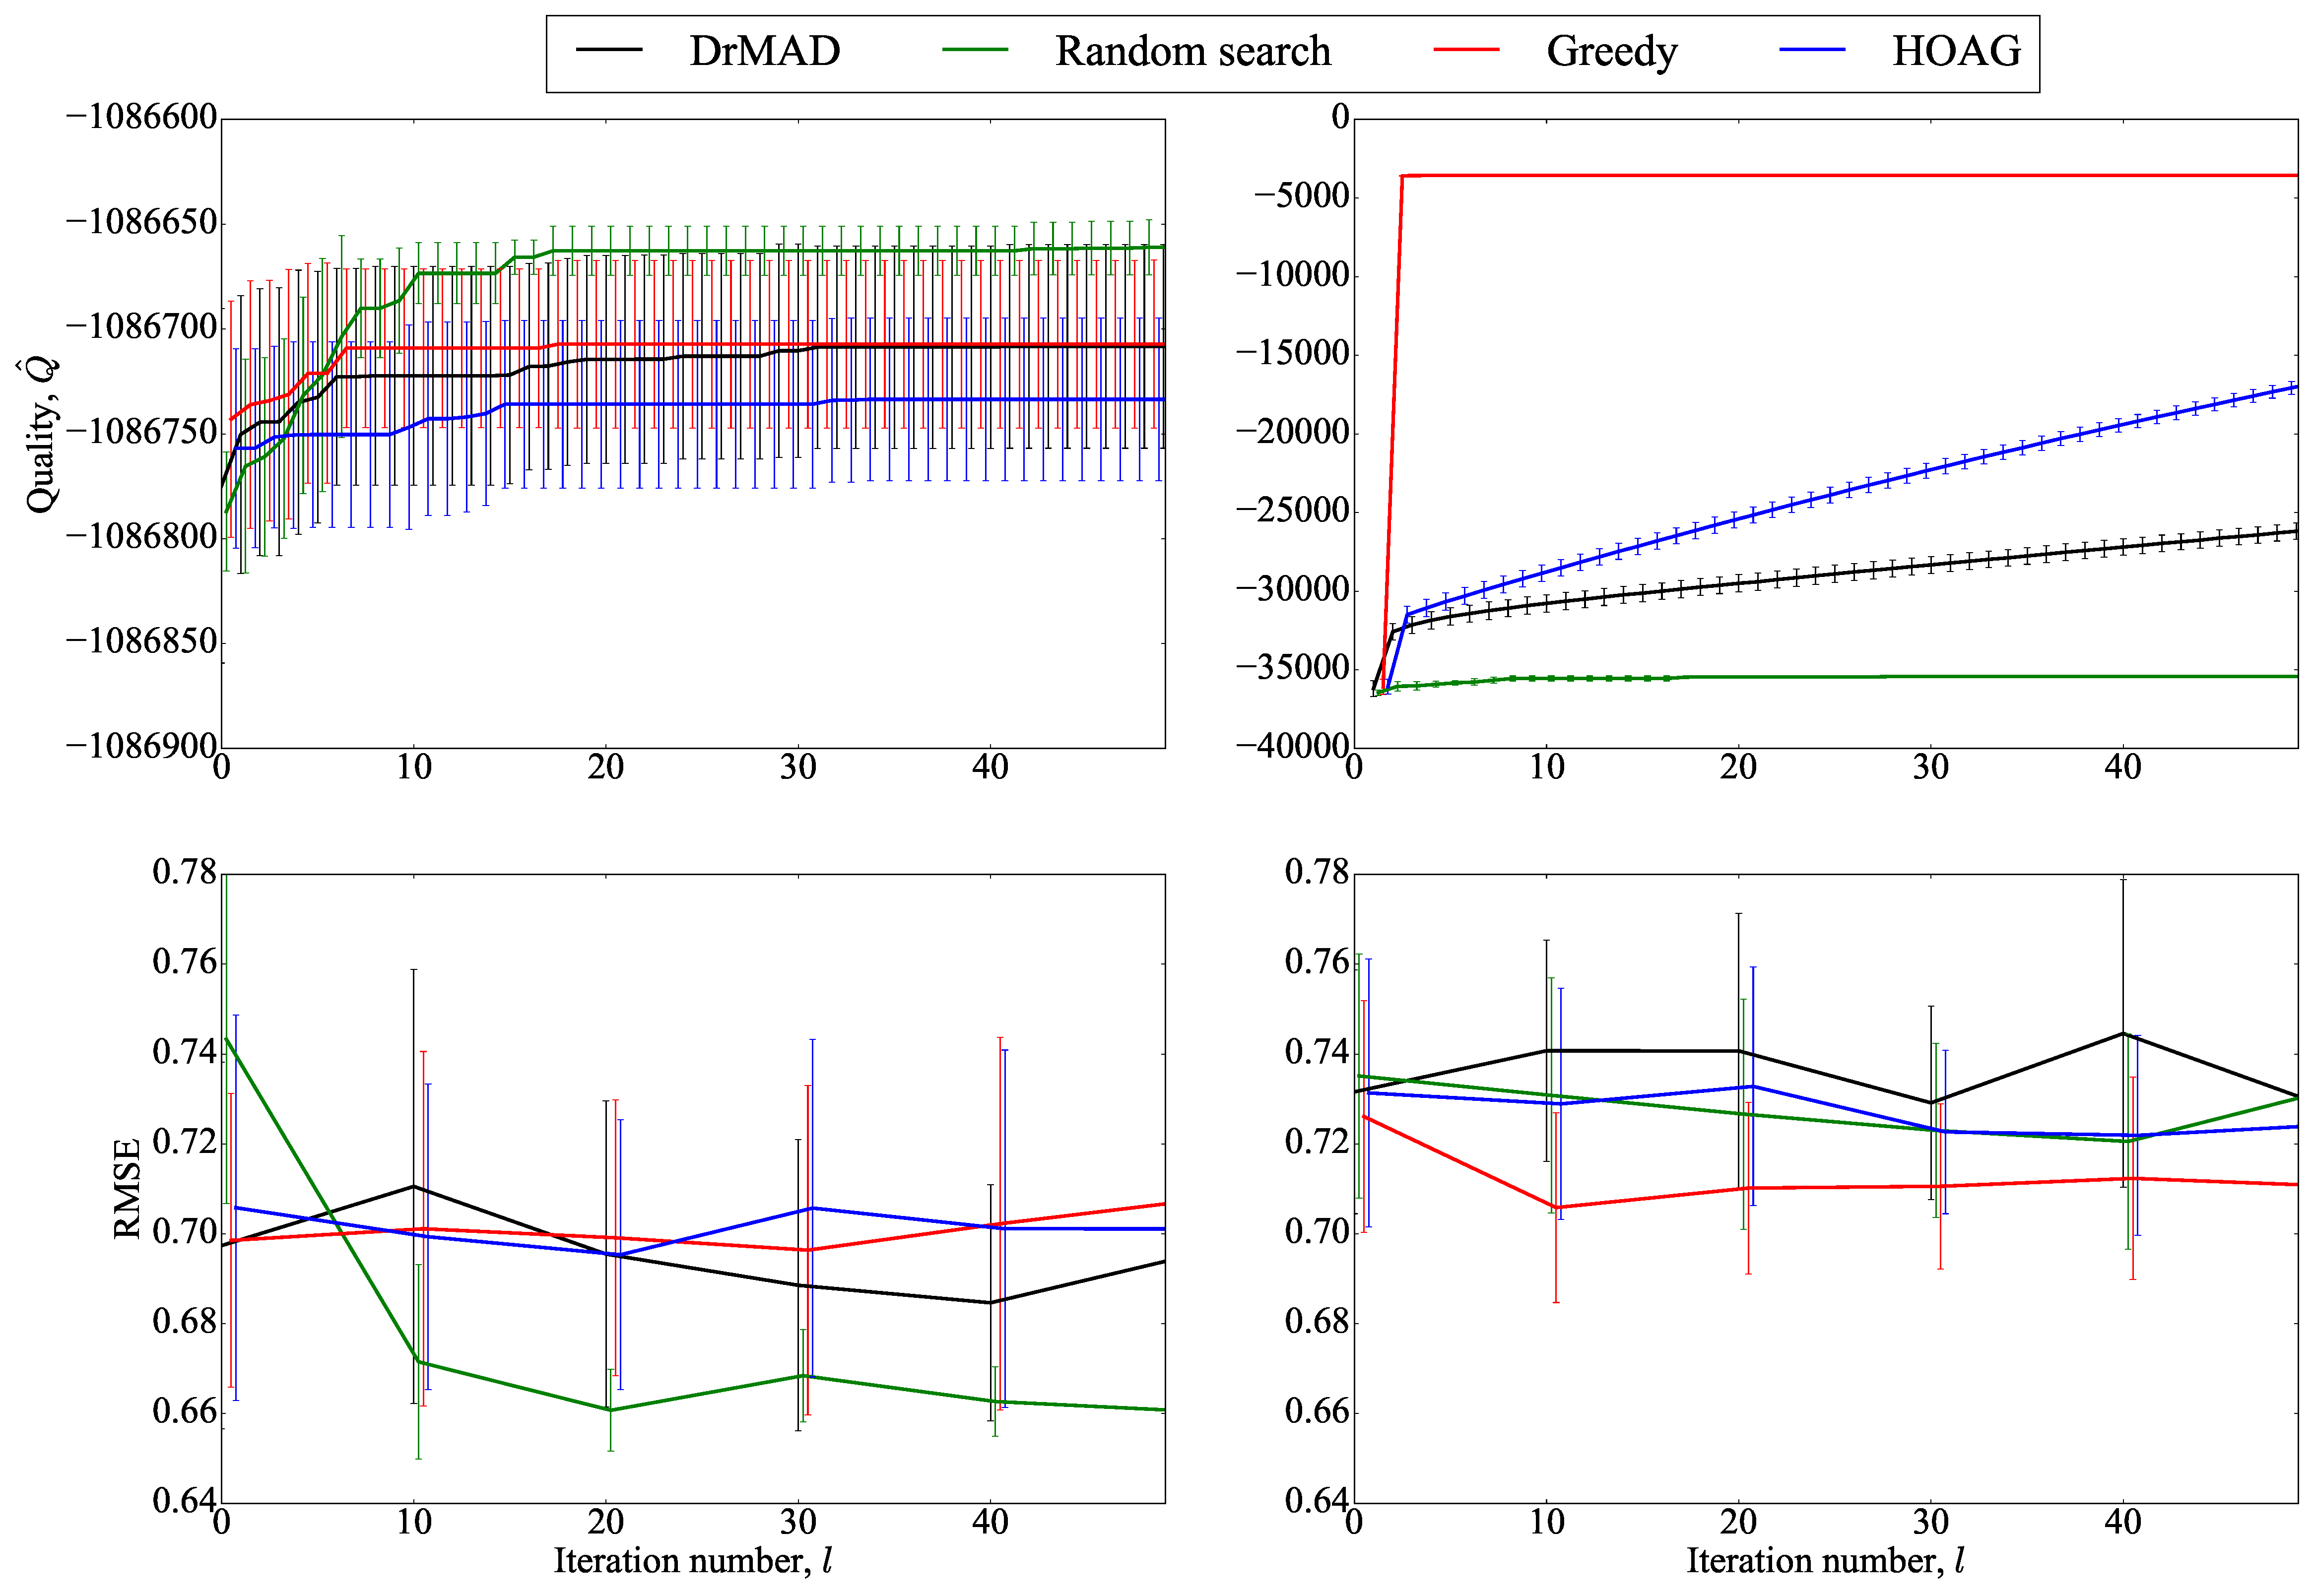
\includegraphics[width=\linewidth]{Fig_wisdm.eps}
\caption{WISDM,  best validation value $\hat{Q}$ and RMSE  for cross-validation (left) and evidence lower bound (right)}    
\label{fig:wisdm}
    
    \end{figure*}


    \begin{figure*}

    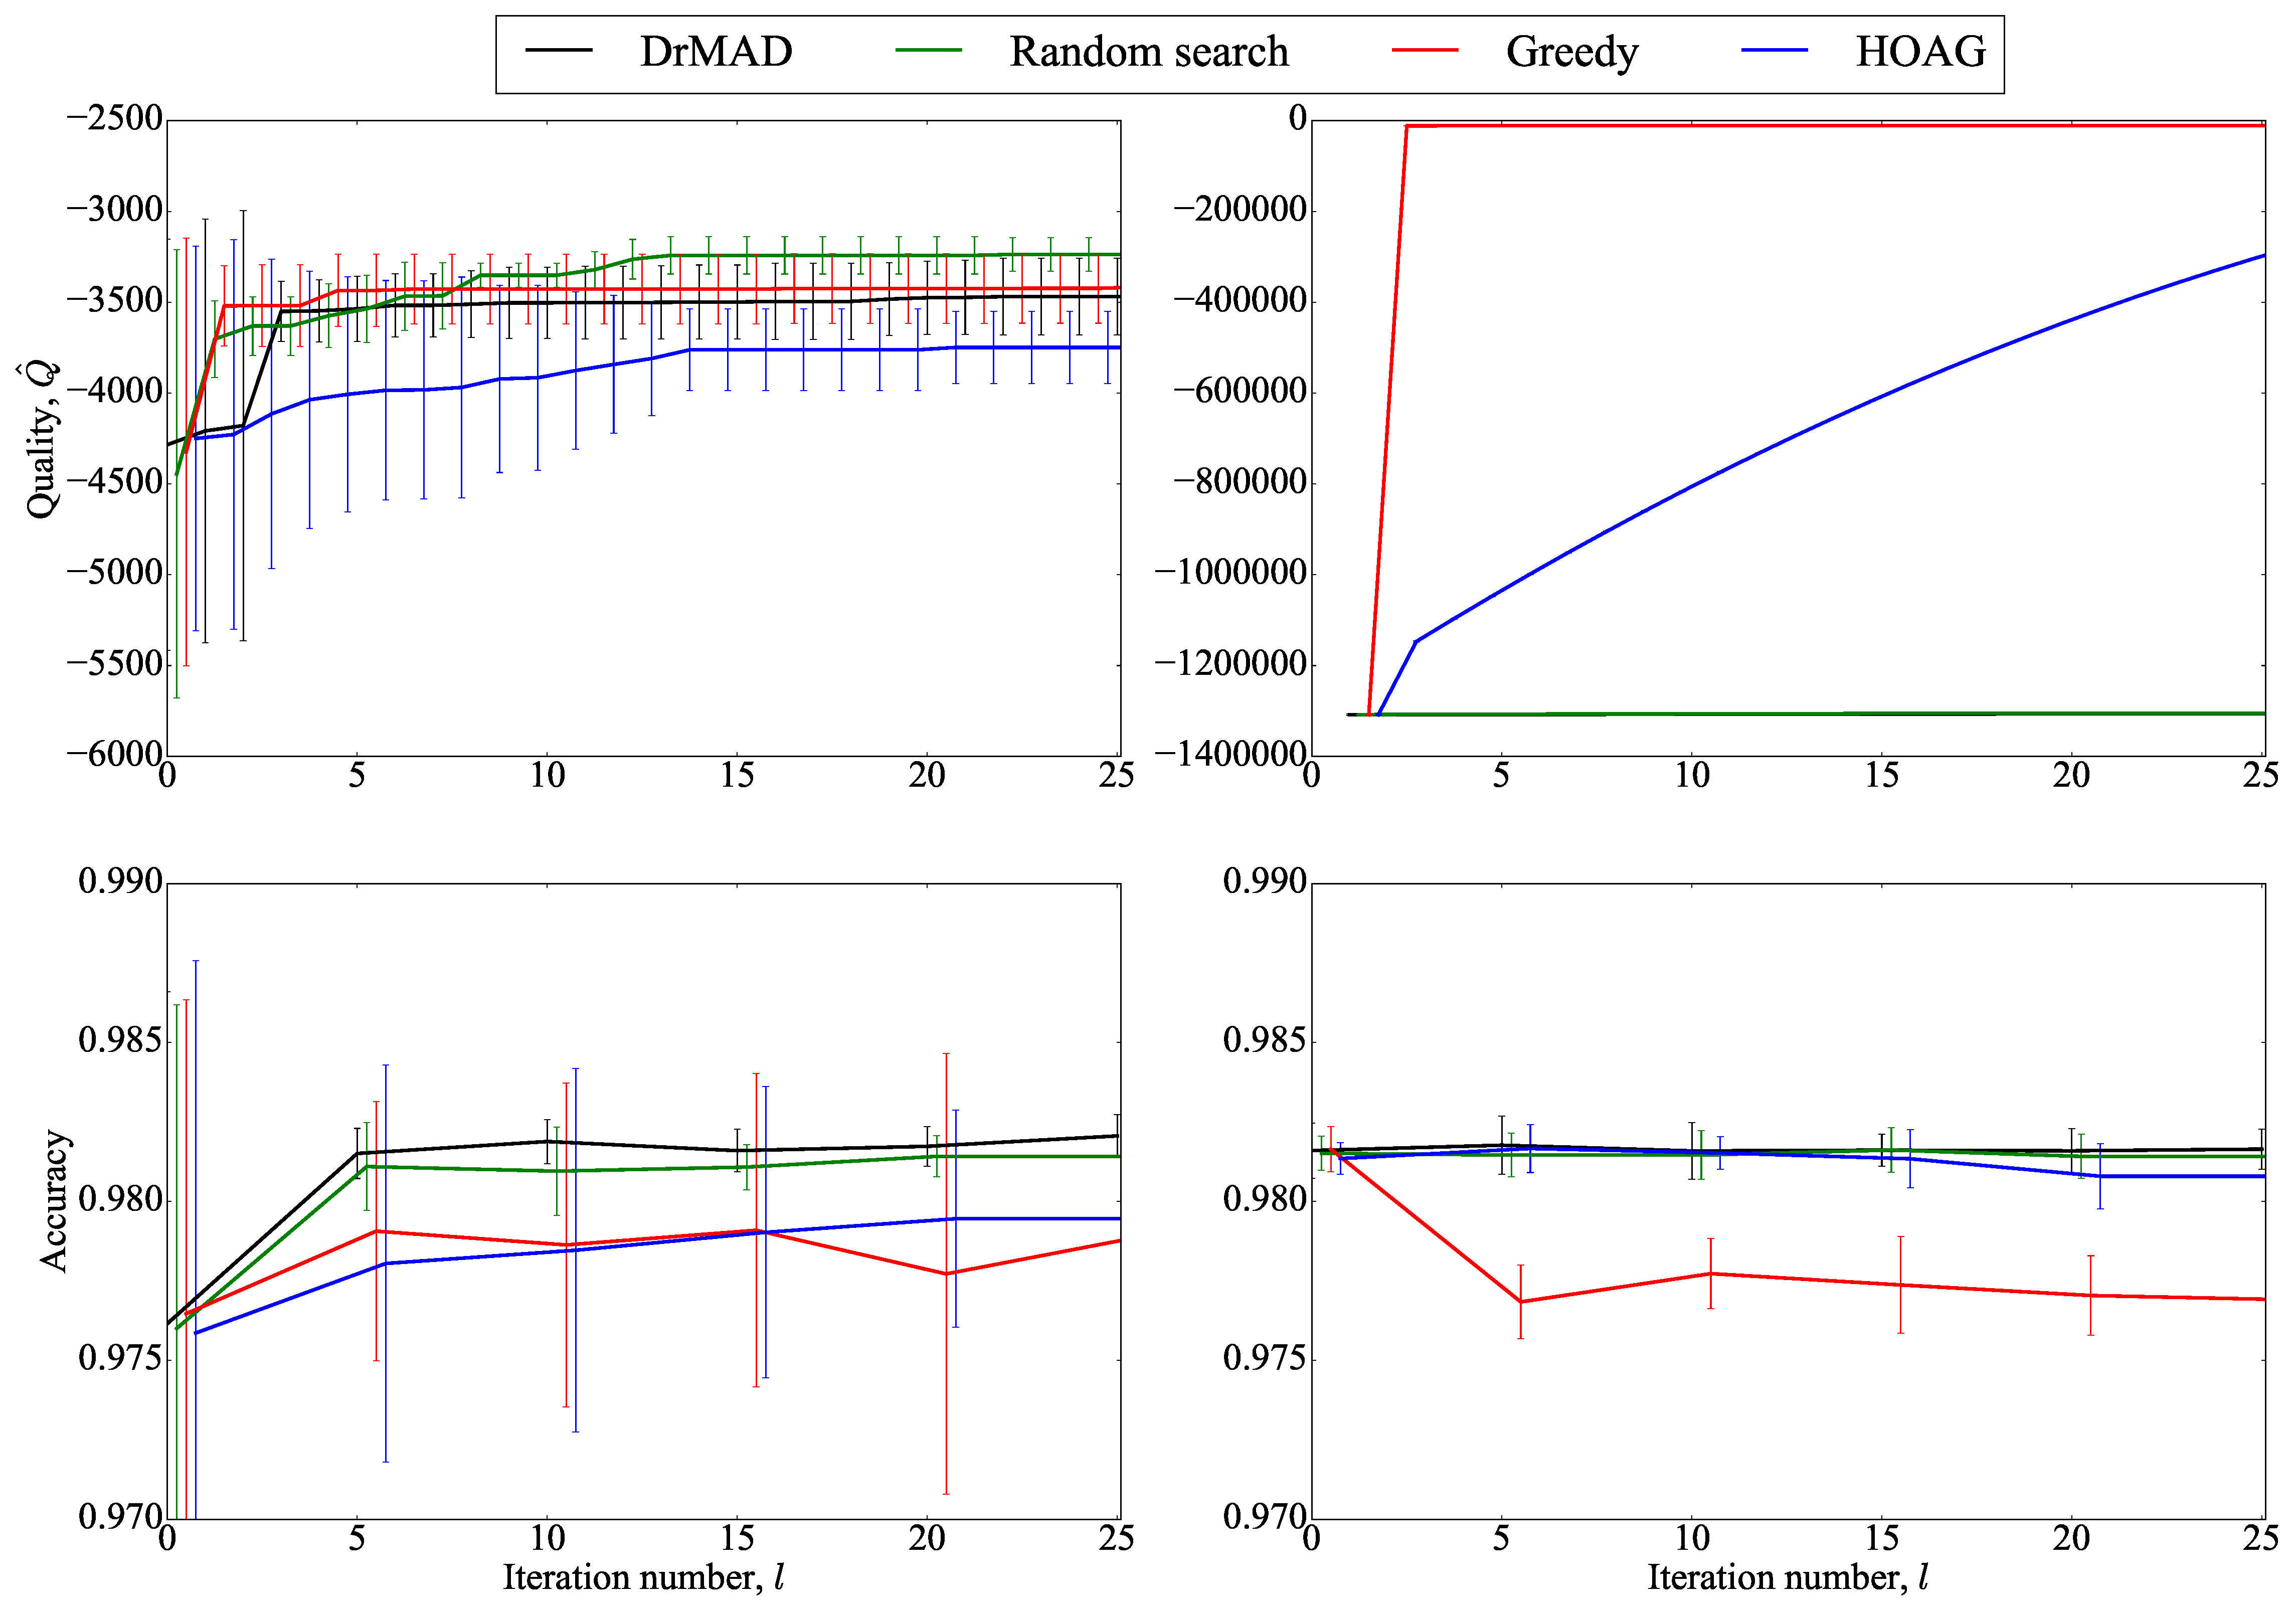
\includegraphics[width=\linewidth]{Fig_mnist.eps}

    \caption{MNIST, best validation value  $\hat{Q}$ and Accuracy  for cross-validation (left) and evidence lower bound (right)}
    \label{fig:mnist}
    \end{figure*}

    \begin{figure*}

    \includegraphics[width=\linewidth]{Fig_noise.pdf}

    \caption{MNIST, Model accuracy with noise in the Test dataset. The hyperparameters were optimized with evidence lower bound criterion.}
    \label{fig:noise}
    \end{figure*}





\section{Discussion}
\label{discussion}
The experiments showed that each algorithm perform effectively and therefore the appropriate hyperparameter optimization method should rely on the amount of hyperparameters and the specific of the problem. 

When dealing with small amount of hyperparameters random search showed the best results since search procedure can be employed more effectively than gradient-based optimization in low-dimensional hyperparameters space. For the high-dimensional hyperparameter space both  HOAG and greedy algorithms showed good performance. 
HOAG algorithm would be more preferable if the model optimization problem is expensive. On the other hand we can schedule greedy hyperparameter optimization to make it less expensive as in~\cite{hyper_greed}. 

DrMad algorithm showed rather poor results on the MNIST and WISDM datasets. Perhaps, it is so because of high learning rate $\gamma$ used in experiments. The large value of the learning rate can make DrMad algorithm instable. Two improvements can be proposed. We can use more stable optimization like Adam or AdaGrad for both parameter and hyperparameter optimization. The second improvement was proposed in~\cite{hyper_mad}: we can use more complicated parameter trajectory approximation to make it more similar to the original parameter trajectory. Opposing to HOAG and greedy algorithms, DrMad optimization has prerequisites for not only hyperparameters optimization but also the metaparameters, i.e. the optimization procedure parameters. The opportunity of such optimization using reversed differentiation was shown in~\cite{hyper_mad}. 

The other interesting aspect of our experiments is the relation between the model error (RMSE or Accuracy) and the value of validation loss $Q$. The models obtained by the evidence lower bound showed higher error rate than the models obtained using cross-validation on the MNIST and WISDM datasets. These models also showed greater stability when noise was added to the Test datasets.  The evidence lower bound showed significantly better results on the synthetic dataset, when the amount of objects in the Train dataset is small. Therefore we conclude that the evidence lower bound usage is preferable when the model tends to overfit or when the cross-validation usage is too computationally expensive.   In~\cite{nips} it is noted that the evidence lower bound optimization required more iterations for the convergence. In our experiments we used the same number of iterations both for the cross-validation and evidence lower bound. The more accurate iteration number calibration can improve the final quality of these models. 

\section{Conclusion and future work}
\label{concl}
The paper analyzed the gradient-based hyperparameter optimization algorithms. We adapted the analyzed algorithms for general validation functions and evaluated their performance on the  MNIST and WISDM datasets. Two model selection criteria were compared: the cross-validation and evidence lower bound. 

The experiments showed that the gradient-based algorithms are effective when the number of hyperparameters is large. The results showed that models obtained using evidence lower bound have higher error rater than models obtained using cross-validation, but they are also more stable when the test dataset contains a lot of noise. 

The authors  implemented these algorithms as a toolbox available at~\cite{pyfos}. The toolbox is developed in Python using Theano~\cite{theano} and Numpy~\cite{numpy} libraries. 

In out future work we are planning to develop the analyzed algorithm and to extend gradient-based algorithms to optimize not only hyperparameters, but also the model optimization parameters. The other object of our future research will is the difference between the cross-validation and evidence lower bound and the theoretical aspects of their properties for the models with large amount of parameters.

%addcontentsline{toc}{section}{References}
\bibliographystyle{spmpsci}
%\bibliographystyle{unsrt}
\bibliography{lit}

\end{document}
